\documentclass{article}
\usepackage{graphicx} % Needed for including graphics
\usepackage{amsmath} % Needed for math formatting like \sigma
\usepackage{caption}

\title{HW 6 Report}
\author{Hunter Garrison}

\begin{document}
\maketitle

\section*{Question 1}

\subsection*{Spectral}
We begin with using spectral clustering on slices of our dataset. We compute both the ARI and SSE of each slice and find which parameters are showing the largest values for ARI and smallest values for SSE. Below are the corresponding plots:

\noindent
\begin{minipage}{.5\textwidth}
  \centering
  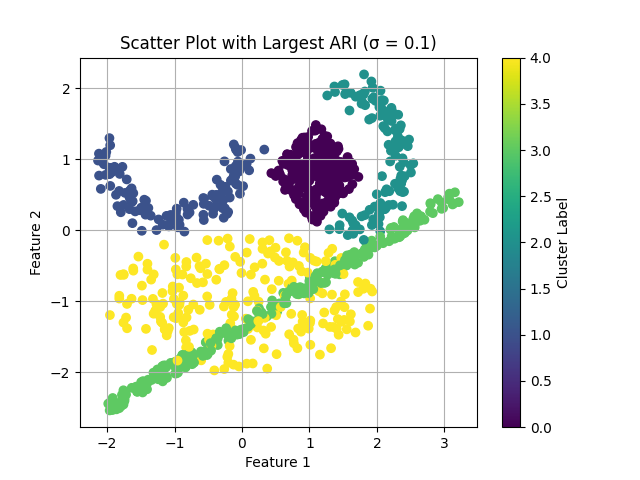
\includegraphics[width=0.9\linewidth]{Spectral_ARI.png}
  \captionof{figure}{Plot of ARI for spectral clustering}
\end{minipage}%
\begin{minipage}{.5\textwidth}
  \centering
  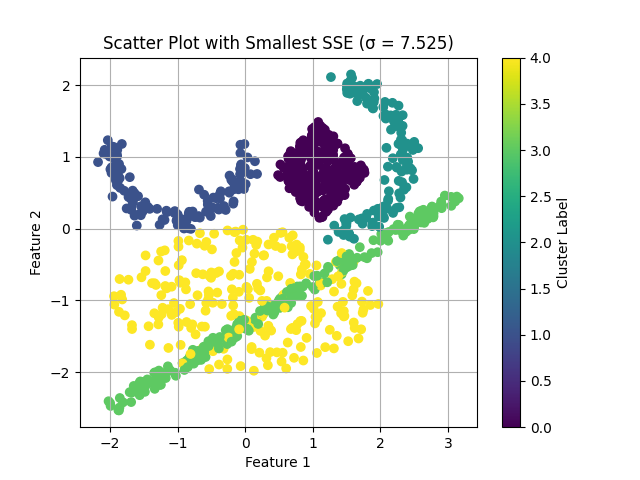
\includegraphics[width=0.9\linewidth]{Spectral_SSE.png}
  \captionof{figure}{Plot of SSE for spectral clustering}
\end{minipage}

As we can see, $\sigma=0.1$ yields the largest ARI and $\sigma=7.525$ yields the smallest SSE.

We now perform spectral clustering on all slices of our dataset and report the eigenvalues. Below is a plot of the eigenvalues:

\noindent
\begin{minipage}{\textwidth}
    \centering
    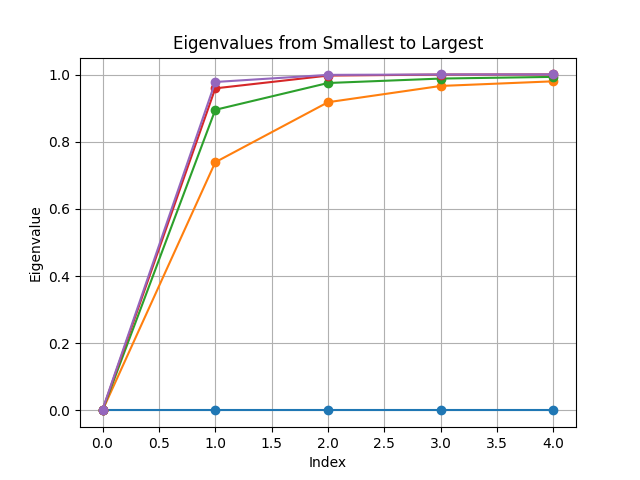
\includegraphics[width=0.5\textwidth]{Spectral_eig.png}
    \captionof{figure}{Plot of eigenvalues from spectral clustering}
\end{minipage}%


\subsection*{Jarvis-Patrick}
We now perform Jarvis-Patrick clustering on slices of our dataset. Similar to before, we compute both the ARI and SSE of each slice and find which parameters are showing the largest values for ARI and smallest values for SSE. Below are the corresponding plots:


\noindent
\begin{minipage}{.5\textwidth}
  \centering
  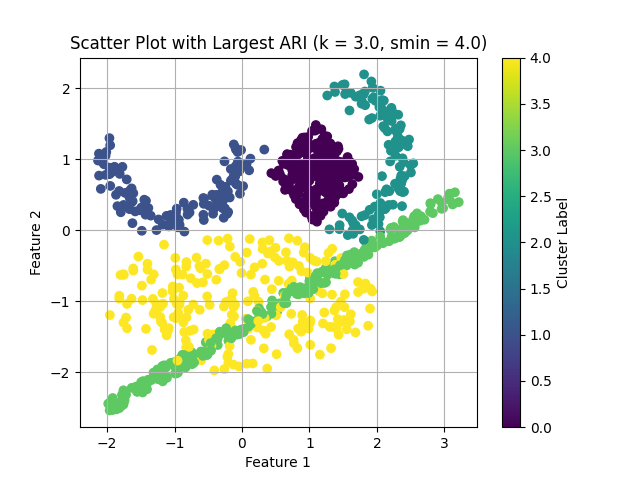
\includegraphics[width=0.9\linewidth]{Jarvis_ARI.png}
  \captionof{figure}{Plot of ARI for Jarvis-Patrick clustering}
\end{minipage}%
\begin{minipage}{.5\textwidth}
  \centering
  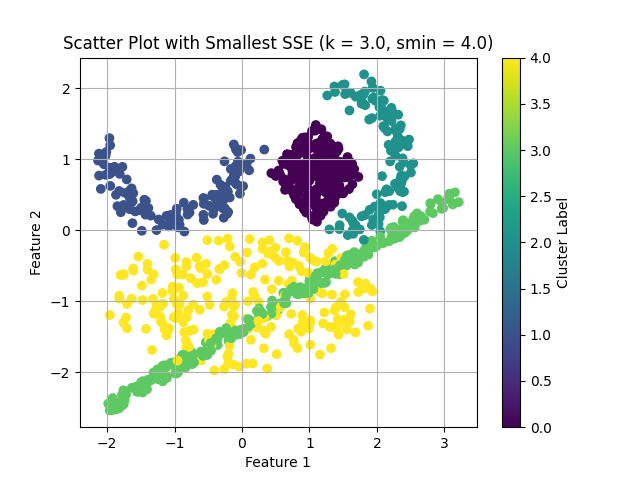
\includegraphics[width=0.9\linewidth]{Jarvis_SSE.png}
  \captionof{figure}{Plot of SSE for Jarvis-Patrick clustering}
\end{minipage}


As we can see, we get the largest ARI with a $k$ value of 3 and a $s_{\text{min}}$ value of 4, and we also get the smallest SSE with the same parameter values.

\section*{Question 2}

We now perform the Expectation Maximization algorithm by creating a Gaussian mixture model. Upon doing so we can find the log likelihood values per iteration as shown below:

\begin{figure}[h]
    \centering
    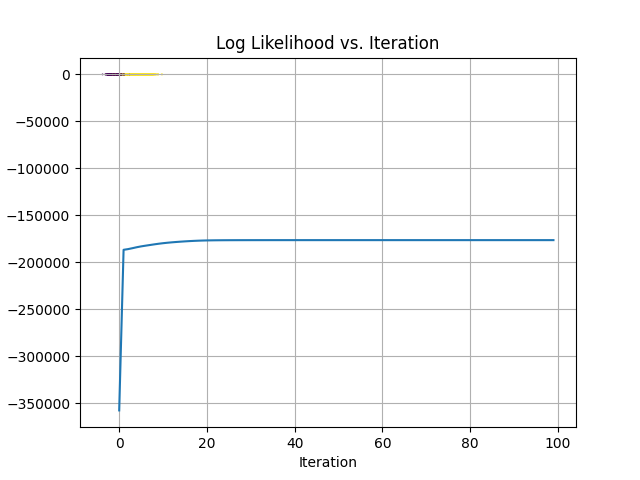
\includegraphics[width=0.5\textwidth]{plot_log_likelihood.png}
    \caption{Plot of log likelihood values per iteration}
\end{figure}

\end{document}

